\section{Graphing \graphing{Using Power Series}}
\subsection{Second Derivative Test via Power Series}
Recall the Second Derivative Test from Calculus I.  
\begin{exercise}{Go Ahead, Recall It \Coffeecup}
State the Second Derivative Test. \vspace*{1in}
\end{exercise}

How does this relate to looking at the degree two power series of a function?  We investigate below.
\begin{exercise}{\secondderivativetest{Power Series Interpretation} of the Second Derivative Test \Coffeecup \Coffeecup}
Let $c$ be a critical point of the function $f(x)$. 
\begin{itemize}
\item If $f''(c)<0$, what does that tell you about the \concavity{degree two power series} for $f(x)$ centered at $c$? Explain. \vspace*{1in}
\item If $f''(c)>0$, what does that tell you about the degree two power series for $f(x)$ centered at $c$? Explain.  \vspace*{1in}
\item When $f''(c)=0$, in Calculus I we would say the \concavity{Second Derivative Test} gave no information.  With power series, how can you get around this situation and figure out the graph's behavior at that point?  \vspace*{1in}
\end{itemize}
\end{exercise}

Let us now put this to work, analyzing a complicated function!
\begin{exercise}{An Ugly Polynomial \Coffeecup \Coffeecup \Coffeecup}
Graph the function by hand $f(x)=36x-30x^2+\frac{28}{3}x^3-x^4$ using the following steps:

\begin{itemize}
\item Determine the end behavior of the function.  That is, figure out the limits as $x$ approaches infinity and minus infinity.
\vspace*{1in}
\item Compute $f(x)$ at the $x$-values $x=0,2,4,6$ and plot those points to get started.
\vspace*{1in}
\item Compute $f'(x)$ and set it equal to zero to find any critical points.
\vspace*{2in}
\item Find the power series of $f(x)$ centered at each of those critical points.  From these series conclude max/min/saddle at each critical point.  
\vspace*{2in}
\item Sketch the graph!
\begin{center}
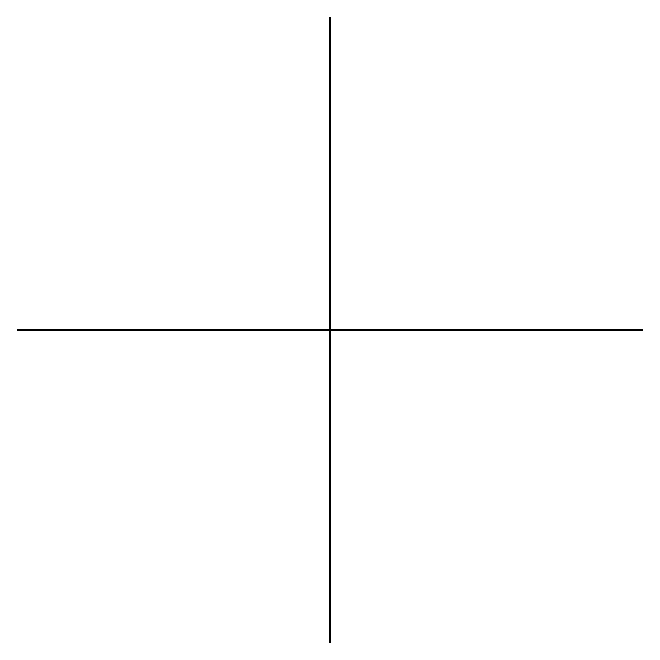
\includegraphics[scale=0.5]{quadall}
\end{center}
\end{itemize}
\end{exercise}

\subsection{Symmetry via Power Series}

One powerful technique in mathematics is the exploitation of symmetry.  In the context of graphing, two commonly used types of symmetry are even symmetry and odd symmetry.  Recall the \oddsymmetry{definition}s of even and odd symmetry below.

\begin{exercise}{Definitions of Even and Odd \Coffeecup}
Complete the \evensymmetry{definition}s.
\begin{itemize}
\item We say a function $f(x)$ has \emph{even} symmetry if and only if... \vspace*{.2in}
\item We say a function $f(x)$ has \emph{odd} symmetry if and only if... \vspace*{.2in}
\end{itemize}
\end{exercise}

\begin{exercise}{Symmetry of Sine and Cosine \Coffeecup \Coffeecup}
\begin{itemize}
\item Use the power series for cosine to prove that cosine has \cosine{even symmetry}.
\vspace*{.5in}
\item Use the \oddsymmetry{power series} for sine to prove that sine has \sine{odd symmetry}.
\vspace*{.5in}
\end{itemize}
\AnswerKeyEntry{Substitute $-x$ into the power series for cosine and simplify to demonstrate that $\cos(-x)=\cos(x)$, and similarly for sine.}
\end{exercise}

As the above exercise demonstrates, the key to a function having even (odd) symmetry is for the \evensymmetry{power series} to only have terms of even (odd) degree!  This not only justifies the names of the types of symmetry, but also gives us a quick and easy way to determine the symmetry of a function.  

\begin{exercise}{Testing Our Known Series for Symmetry \Coffeecup \Coffeecup}
Scan through our list of known power series.  Classify each function as odd, even, or neither.  List any symmetries that you found below!
\vspace*{2in}
\end{exercise}